%package list
\documentclass{article}
\usepackage[top=3cm, bottom=3cm, outer=3cm, inner=3cm]{geometry}
\usepackage{multicol}
\usepackage{listings}
\usepackage[utf8]{inputenc}
\usepackage{graphicx}
\usepackage{url}
%\usepackage{cite}
\usepackage{hyperref}
\usepackage{array}
%\usepackage{multicol}
\newcolumntype{x}[1]{>{\centering\arraybackslash\hspace{0pt}}p{#1}}
\usepackage{natbib} 
\usepackage{pdfpages}
\usepackage{multirow}   
\usepackage[normalem]{ulem}
\useunder{\uline}{\ul}{}
\usepackage{svg}
\usepackage{xcolor}
\usepackage{listings}
\lstdefinestyle{ascii-tree}{
    literate={├}{|}1 {─}{--}1 {└}{+}1 
  }
\lstset{basicstyle=\ttfamily,
  showstringspaces=false,
  commentstyle=\color{red},
  keywordstyle=\color{blue}
}
%\usepackage{booktabs}
\usepackage{caption}
\usepackage{subcaption}
\usepackage{float}
\usepackage{array}

\newcolumntype{M}[1]{>{\centering\arraybackslash}m{#1}}
\newcolumntype{N}{@{}m{0pt}@{}}


%%%%%%%%%%%%%%%%%%%%%%%%%%%%%%%%%%%%%%%%%%%%%%%%%%%%%%%%%%%%%%%%%%%%%%%%%%%%
%%%%%%%%%%%%%%%%%%%%%%%%%%%%%%%%%%%%%%%%%%%%%%%%%%%%%%%%%%%%%%%%%%%%%%%%%%%%
\newcommand{\itemEmail}{ shanccom@unsa.edu.pe \newline
ynoa@unsa.edu.pe
}
\newcommand{\itemStudent}{ Sergio Hancco Mullisaca \newline
Noa Camino Yenaro Joel}
\newcommand{\itemCourse}{Programacion Web 2}
\newcommand{\itemCourseCode}{}
\newcommand{\itemSemester}{II}
\newcommand{\itemUniversity}{Universidad Nacional de San Agustín de Arequipa}
\newcommand{\itemFaculty}{Facultad de Ingeniería de Producción y Servicios}
\newcommand{\itemDepartment}{Departamento Académico de Ingeniería de Sistemas e Informática}
\newcommand{\itemSchool}{Escuela Profesional de Ingeniería de Sistemas}
\newcommand{\itemAcademic}{2024 - A}
\newcommand{\itemInput}{Del 16 Mayo 2024}
\newcommand{\itemOutput}{Al 18 Mayo 2024}
\newcommand{\itemPracticeNumber}{4}
\newcommand{\itemTheme}{AJAX}
%%%%%%%%%%%%%%%%%%%%%%%%%%%%%%%%%%%%%%%%%%%%%%%%%%%%%%%%%%%%%%%%%%%%%%%%%%%%
%%%%%%%%%%%%%%%%%%%%%%%%%%%%%%%%%%%%%%%%%%%%%%%%%%%%%%%%%%%%%%%%%%%%%%%%%%%%

\usepackage[english,spanish]{babel}
\usepackage[utf8]{inputenc}
\AtBeginDocument{\selectlanguage{spanish}}
\renewcommand{\figurename}{Figura}
\renewcommand{\refname}{Referencias}
\renewcommand{\tablename}{Tabla} %esto no funciona cuando se usa babel
\AtBeginDocument{%
	\renewcommand\tablename{Tabla}
}

\usepackage{fancyhdr}
\pagestyle{fancy}
\fancyhf{}
\setlength{\headheight}{30pt}
\renewcommand{\headrulewidth}{1pt}
\renewcommand{\footrulewidth}{1pt}
\fancyhead[L]{\raisebox{-0.2\height}{\includegraphics[width=3cm]{logo_episunsa.png}}}
\begin{figure}
    \centering
    \label{fig:enter-label}
\end{figure}
\fancyhead[C]{\fontsize{7}{7}\selectfont	\itemUniversity \\ \itemFaculty \\ \itemDepartment \\ \itemSchool \\ \textbf{\itemCourse}}
\fancyhead[R]{\raisebox{-0.2\height}{\includegraphics[width=1.2cm]{}}}
\fancyfoot[C]{\itemCourse}
\fancyfoot[R]{Página \thepage}

% para el codigo fuente
\usepackage{listings}
\usepackage{color, colortbl}
\definecolor{dkgreen}{rgb}{0,0.6,0}
\definecolor{gray}{rgb}{0.5,0.5,0.5}
\definecolor{mauve}{rgb}{0.58,0,0.82}
\definecolor{codebackground}{rgb}{0.95, 0.95, 0.92}
\definecolor{tablebackground}{rgb}{0.8, 0, 0}

\lstset{frame=tb,
	language=bash,
	aboveskip=3mm,
	belowskip=3mm,
	showstringspaces=false,
	columns=flexible,
	basicstyle={\small\ttfamily},
	numbers=none,
	numberstyle=\tiny\color{gray},
	keywordstyle=\color{blue},
	commentstyle=\color{dkgreen},
	stringstyle=\color{mauve},
	breaklines=true,
	breakatwhitespace=true,
	tabsize=3,
	backgroundcolor= \color{codebackground},
}

\begin{document}
	
	\vspace*{10px}
	
	\begin{center}	
		\fontsize{17}{17} \textbf{ Informe de Laboratorio \itemPracticeNumber}
	\end{center}
	\centerline{\textbf{\Large Tema: \itemTheme}}
	%\vspace*{0.5cm}	

	\begin{flushright}
		\begin{tabular}{|M{2.5cm}|N|}
			\hline 
			\rowcolor{tablebackground}
			\color{white} \textbf{Nota}  \\
			\hline 
			     \\[30pt]
			\hline 			
		\end{tabular}
	\end{flushright}	

	\begin{table}[H]
		\begin{tabular}{|x{4.7cm}|x{4.8cm}|x{4.8cm}|}
			\hline 
			\rowcolor{tablebackground}
			\color{white} \textbf{Estudiante} & \color{white}\textbf{Escuela}  & \color{white}\textbf{Asignatura}   \\
			\hline 
			{\itemStudent \par \itemEmail} & \itemSchool & {\itemCourse \par Semestre: \itemSemester \par Código: \itemCourseCode}     \\
			\hline 			
		\end{tabular}
	\end{table}		
	
	\begin{table}[H]
		\begin{tabular}{|x{4.7cm}|x{4.8cm}|x{4.8cm}|}
			\hline 
			\rowcolor{tablebackground}
			\color{white}\textbf{Laboratorio} & \color{white}\textbf{Tema}  & \color{white}\textbf{Duración}   \\
			\hline 
			\itemPracticeNumber  & \itemTheme & 04 horas   \\
			\hline 
		\end{tabular}
	\end{table}
	
	\begin{table}[H]
		\begin{tabular}{|x{4.7cm}|x{4.8cm}|x{4.8cm}|}
			\hline 
			\rowcolor{tablebackground}
			\color{white}\textbf{Semestre académico} & \color{white}\textbf{Fecha de inicio}  & \color{white}\textbf{Fecha de entrega}   \\
			\hline 
			\itemAcademic & \itemInput &  \itemOutput  \\
			\hline 
		\end{tabular}
	\end{table}
	
	\section{Tarea}
	\begin{itemize}		
		\item Informe de laboratorio
            \item Video en Flip
		\item Ejercicios Propuestos
            \item Ejercicios
        
	\end{itemize}
		
	\section{Equipos, materiales y temas utilizados}
	\begin{itemize}
		\item VS
		\item Git 2.39.2.
		\item Cuenta en GitHub con el correo institucional.
	\end{itemize}
    \clearpage
    
	\section{URL de Repositorio Github}
	\begin{itemize}
        \item URL del video en yt.
		\item \url{https://youtu.be/nc4tQ6ytBUw}
        \item URL del video en flip.
		\item \url{https://flip.com/s/VeHz2Bb6FT_c}
        \item URL del GITHUB.
            \item \url{https://github.com/shanccom/Programacion_Web_2.git}
		\item \url{https://github.com/ynoacamino/pweb2}
	\end{itemize}
	
	\section{Actividades}
	\subsection{W3school}

        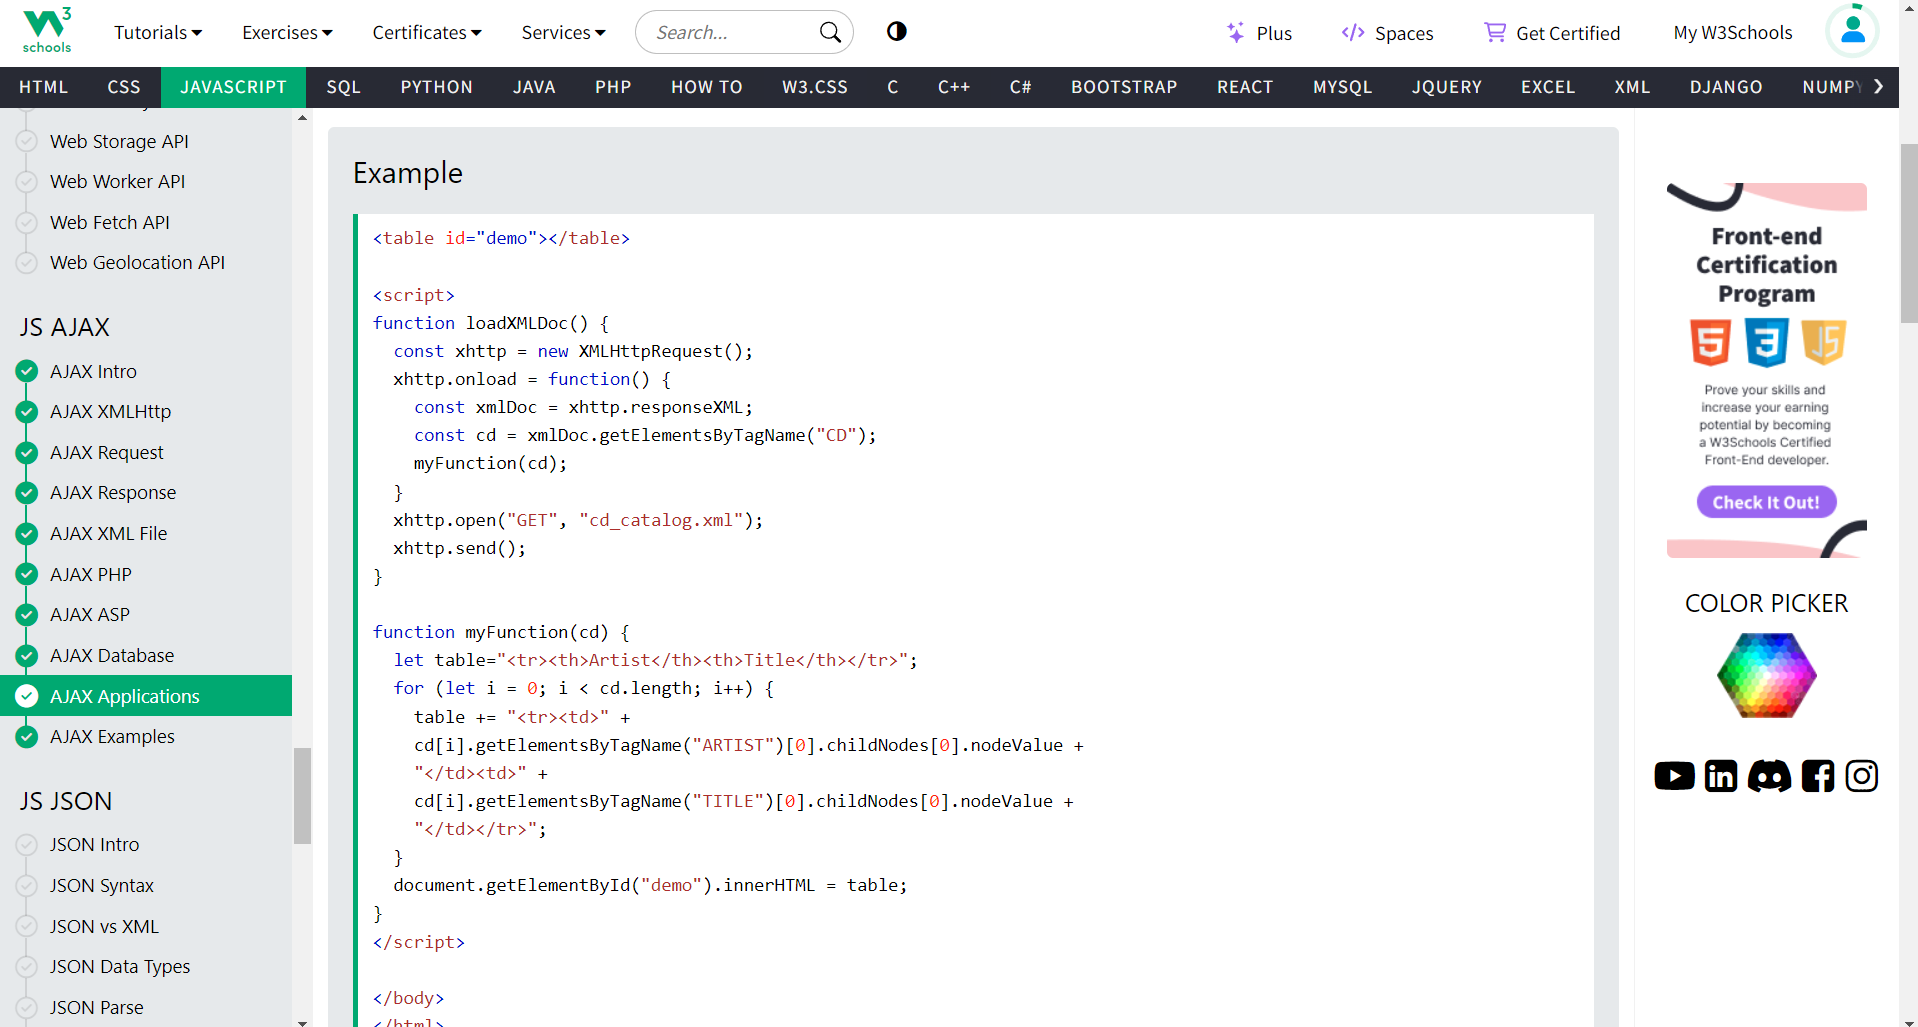
\includegraphics[width=0.8\textwidth,keepaspectratio]{informes/w3school.png}
        
	\subsection{Ejercicios Propuestos}
	\begin{itemize}	
 
		\item Listar los archivos Markdown disponibles
            \item Ver el contenido de un archivo Markdown traducido a HTML
            \item Crear nuevos archivos MarkDown y almacenarlos en el servidor


            \begin{lstlisting}[language=JavaScript, caption=EJERCICIOS PROPUESTOS]

const express = require('express');
const Markdown = require('markdown-it');
const fs = require("node:fs");
const { request } = require('node:http');
const path = require("node:path")
const bodyParser = require('body-parser');

const md = new Markdown();

const app = express();

app.use(express.static('public'));
app.use(bodyParser.urlencoded({extended: false}));

app.get('/', (request, response) => {
  response.send('Hola mundo');
})

app.get('/list', (request, response) => {
  response.send(`
    <ul>
      <li><a href="/primero.md">Markdown 1</a></li>
      <li><a href="/segundo.md">Markdown 2</a></li>
      <li><a href="/tercero.md">Markdown 3</a></li>
    </ul>
  `);
})

app.get('/html', (request, response) => {
  fs.readFile(path.join(__dirname, "public", "primero.md"), {encoding: "utf-8"}, (err, data) => {
    if (err) {
      response.send("Error al leer el archivo");
      return;
    }

    const htmlCode = md.render(data);

    response.send(htmlCode);
  })
})

app.get('/upload', (request, response) => {
  response.sendFile(path.join(__dirname, "public", "upload.html"));
});
app.post("/upload", async (request, response) => {
  const body = request.body;

  const { title, content } = body;

  fs.writeFile(path.join(__dirname, "public", title + ".md"), content, (err) => {
    if (err) {
      response.send("Error al guardar el archivo");
      return;
    }

    response.send(`Archivo guardado correctamente visitelo <a href='/${title}.md'>aqui</a>`);
  })

});


app.listen(3000, () => {
  console.log('Servidor escuchando en http://localhost:3000/')
})


            \end{lstlisting}            
            \item HTML usado para la ejecucion del codigo.
            
            \begin{lstlisting}[language=JavaScript, caption=HTML PARA LOS EJERCICIOS PROPUIESTOS ]
<!DOCTYPE html>
<html lang="en">
<head>
  <meta charset="UTF-8">
  <meta name="viewport" content="width=device-width, initial-scale=1.0">
  <title>Subida de markdowns</title>
</head>
<body>
  <form action="/upload" method="POST">
    <label for="title">Título</label>
    <input type="text" name="title" id="title">
    <label for="content">Contenido</label>
    <textarea name="content" id="content" cols="30" rows="10"></textarea>
    <button type="submit">Enviar</button>
  </form>
</body>
</html>

            \end{lstlisting} 
            
            \newline \newline \newline
        
            \subsection{Ejercicios}
            
            \item Liste todas las “regiones”.

            \begin{lstlisting}[language=JavaScript, caption=PROBLEMA1-INDEX]
            <!DOCTYPE html>
<html lang="en">
<head>
  <meta charset="UTF-8">
  <meta name="viewport" content="width=, initial-scale=1.0">
  <title>Problema 1</title>
</head>
<body>
  <h1>Problema 1</h1>
  <div id="container">

  </div>
  <script src="./script.js"></script>
</body>
</html>
            \end{lstlisting}  

            \begin{lstlisting}[language=JavaScript, caption=PROBLEMA1-SCRIPT]
const $container = document.getElementById('container');

const xhr = new XMLHttpRequest(); 

xhr.open('GET', 'http://localhost:8000/data', true);
xhr.onreadystatechange = function () {
  if(xhr.readyState === 4 && xhr.status === 200) {
    const json = JSON.parse(xhr.responseText);
    json.forEach((region) => {
      const $region = document.createElement('div');
      $region.textContent = region.region;
      $container.appendChild($region);
    })
  }
}

xhr.send();
            \end{lstlisting}  

            \newline \newline \newline
            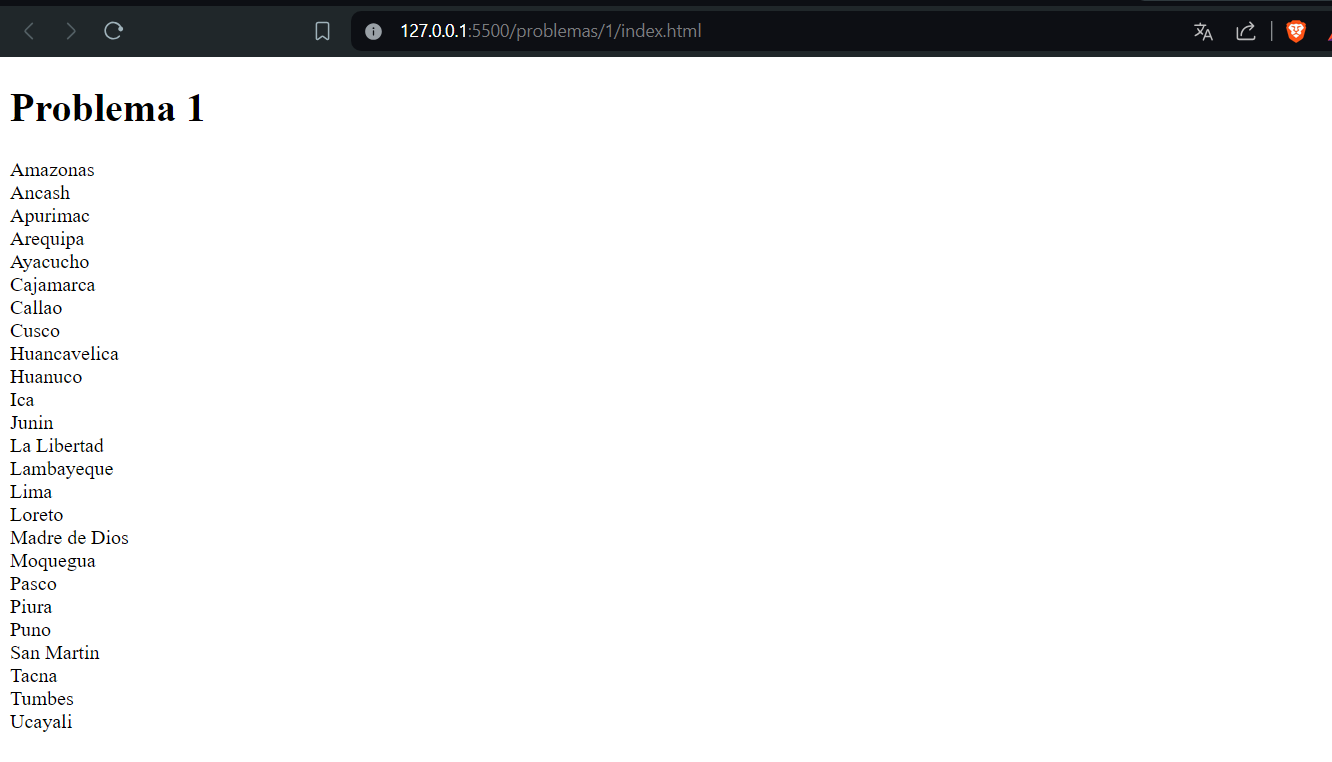
\includegraphics[width=0.8\textwidth,keepaspectratio]{PROBLEMA1.png}
            \newline \newline \newline


            \item Muestre el número total de confirmados por región.

            \begin{lstlisting}[language=JavaScript, caption=PROBLEMA2-INDEX]
<!DOCTYPE html>
<html lang="en">
<head>
  <meta charset="UTF-8">
  <meta name="viewport" content="width=device-width, initial-scale=1.0">
  <title>Problema 1</title>
</head>
<body>
  <h1>Número total de confirmados por región</h1>
  <div id="container">

  </div>
  <script src="./script.js"></script>
</body>
</html>
            \end{lstlisting}  

            \begin{lstlisting}[language=JavaScript, caption=PROBLEMA2-SCRIPT]
const $container = document.getElementById('container');

const xhr = new XMLHttpRequest(); 

xhr.open('GET', 'http://localhost:8000/data', true);
xhr.onreadystatechange = function () {
  if(xhr.readyState === 4 && xhr.status === 200) {
    const data = JSON.parse(xhr.responseText);

    for (const region of data) {
      const $region = document.createElement('div');

      let totalConfirmados = 0;
      for (const confirmado of region.confirmed) {
        totalConfirmados += parseInt(confirmado.value);
      }

      $region.textContent = `${region.region}: ${totalConfirmados} confirmados`;
      
      $container.appendChild($region);
    }
  }
}

xhr.send();
            \end{lstlisting}  

            \newline \newline \newline
            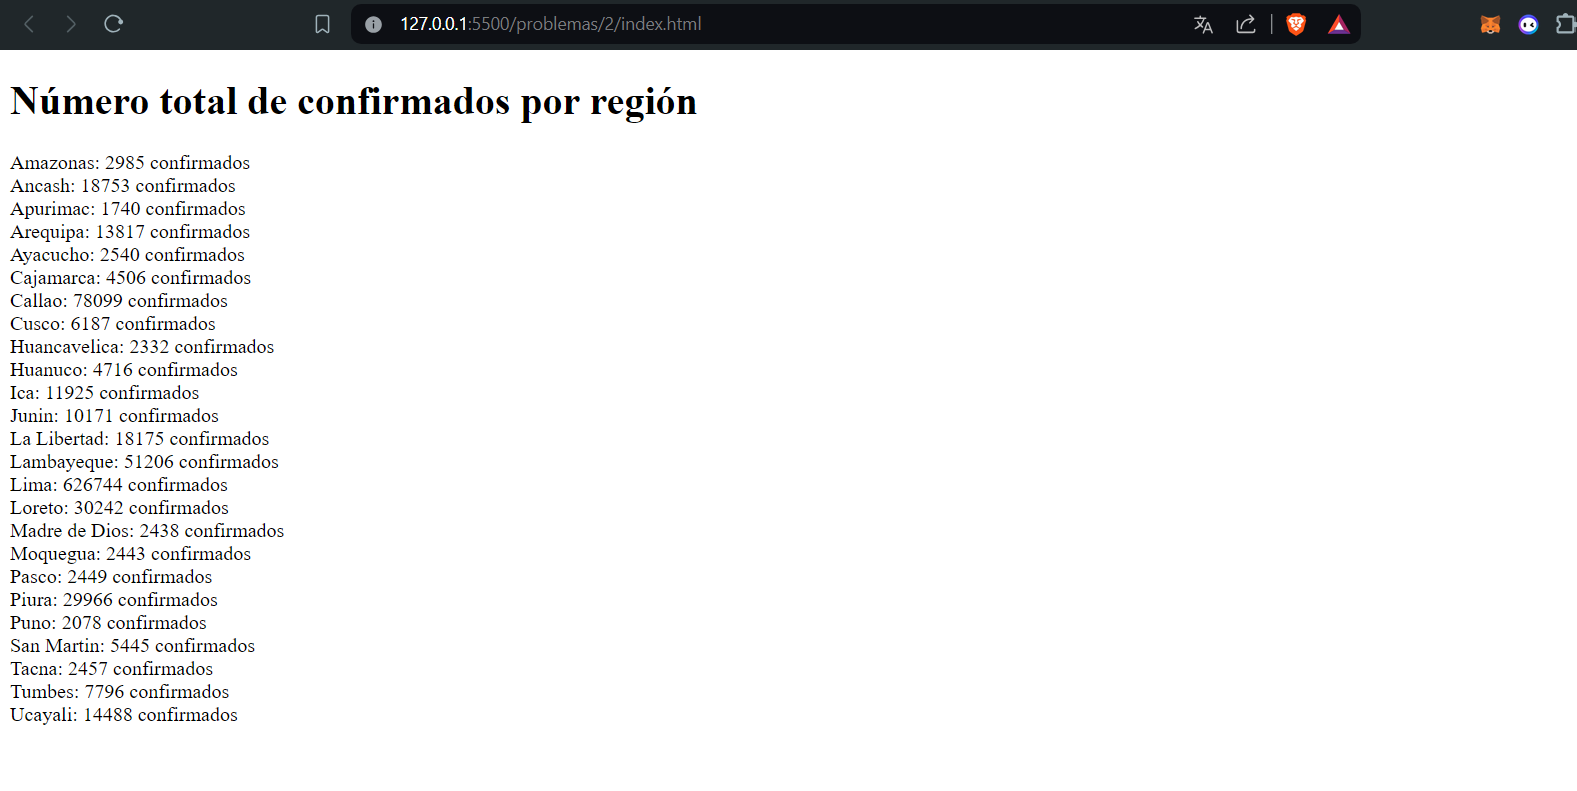
\includegraphics[width=0.8\textwidth,keepaspectratio]{PROBLEMA2.png}
            \newline \newline \newline

            \item Encuentre las 10 regiones cuya suma total sea la mayor.
            
            \begin{lstlisting}[language=JavaScript, caption=PROBLEMA3-INDEX]
<!DOCTYPE html>
<html lang="en">
<head>
  <meta charset="UTF-8">
  <meta name="viewport" content="width=device-width, initial-scale=1.0">
  <title>Top 10 Regiones con Mayor Número de Confirmados</title>
</head>
<body>
  <h1>Top 10 Regiones con Mayor Número de Confirmados</h1>
  <div id="container">

  </div>
  <script src="./script.js"></script>
</body>
</html>
            \end{lstlisting}  

            \begin{lstlisting}[language=JavaScript, caption=PROBLEMA3-SCRIPT]
const $container = document.getElementById('container');

const xhr = new XMLHttpRequest(); 

xhr.open('GET', 'http://localhost:8000/data', true);
xhr.onreadystatechange = function () {
  if(xhr.readyState === 4 && xhr.status === 200) {
    const data = JSON.parse(xhr.responseText);

    const regionSumas = [];
    for (const region of data) {
      let totalConfirmados = 0;
      for (const confirmado of region.confirmed) {
        totalConfirmados += parseInt(confirmado.value);
      }
      regionSumas.push({ region: region.region, total: totalConfirmados });
    }

    regionSumas.sort((a, b) => b.total - a.total);

    for (let i = 0; i < 10; i++) {
      const $region = document.createElement('div');
      $region.textContent = `${i + 1}. ${regionSumas[i].region}: ${regionSumas[i].total} confirmados`;
      $container.appendChild($region);
    }
  }
}

xhr.send();
            \end{lstlisting}  

            \newline \newline \newline
            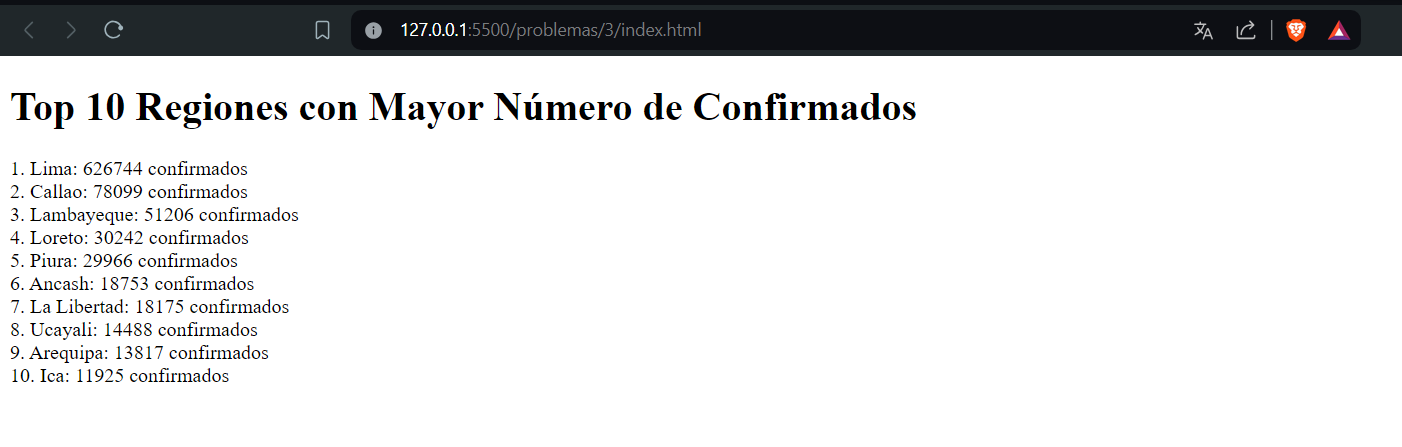
\includegraphics[width=0.8\textwidth,keepaspectratio]{PROBLEMA3.png}
            \newline \newline \newline

            \item Visualice un gráfico en el tiempo de los valores para la región de Arequipa
            
            \begin{lstlisting}[language=JavaScript, caption=PROBLEMA4-INDEX]
<!DOCTYPE html>
<html lang="en">
<head>
  <meta charset="UTF-8">
  <meta name="viewport" content="width=device-width, initial-scale=1.0">
  <title>Problema 4</title>
  <script type="text/javascript" src="https://www.gstatic.com/charts/loader.js"></script>
</head>
<body>
  <h1>
    Problema 4
  </h1>
  <div id="chart_div"></div>
  <script src="./script.js"></script>
</body>
</html>
            \end{lstlisting}  

            \begin{lstlisting}[language=JavaScript, caption=PROBLEMA4-SCRIPT]
const $container = document.getElementById('container');

const xhr = new XMLHttpRequest(); 

xhr.open('GET', 'http://localhost:8000/data', true);
xhr.onreadystatechange = function () {
  if(xhr.readyState === 4 && xhr.status === 200) {
    const json = JSON.parse(xhr.responseText);
    
    const arequipa = json.find((region) => region.region === 'Arequipa');

    google.charts.load('current', {packages: ['corechart', 'line']});
    google.charts.setOnLoadCallback(drawBasic);

    function drawBasic() {
      var data = new google.visualization.DataTable();
      data.addColumn('number', 'X');
      data.addColumn('number', 'Arequipa');

      data.addRows(arequipa.confirmed.map((confirmed, index) => [index, Number(confirmed.value)]));

      var options = {
        hAxis: {
          title: 'Tiempo'
        },
        vAxis: {
          title: 'Infectados'
        }
      };

      var chart = new google.visualization.LineChart(document.getElementById('chart_div'));

      chart.draw(data, options);
    }
  }
}

xhr.send();
            \end{lstlisting}  

            \newline \newline \newline
            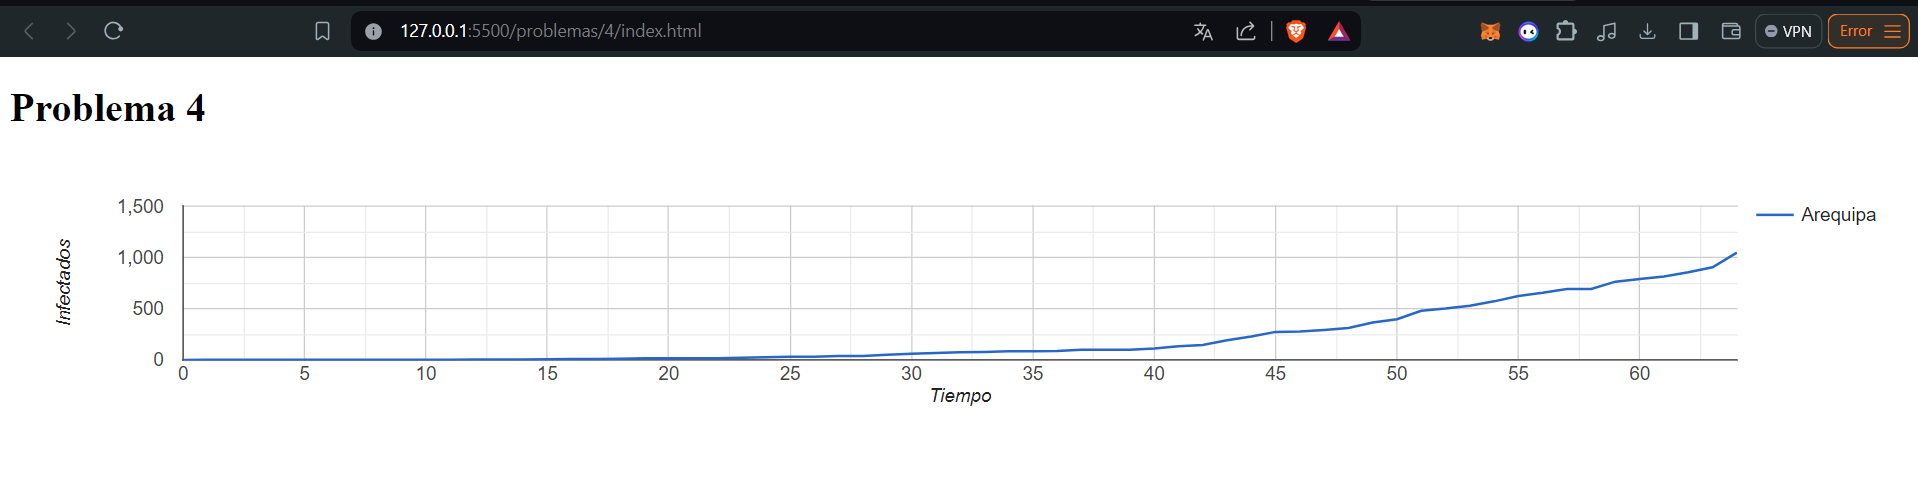
\includegraphics[width=0.8\textwidth,keepaspectratio]{PROBLEMA4.png}
            \newline \newline \newline

            \item Haga gráficos comparativos entre regiones usando líneas.
            
            \begin{lstlisting}[language=JavaScript, caption=PROBLEMA5-INDEX]
<!DOCTYPE html>
<html lang="en">
<head>
  <meta charset="UTF-8">
  <meta name="viewport" content="width=device-width, initial-scale=1.0">
  <title>Problema 5</title>
  <script type="text/javascript" src="https://www.gstatic.com/charts/loader.js"></script>
</head>
<body>
  <h1>Problema 5</h1>
  <div id="chart_div"></div>
  <script src="./script.js"></script>
</body>
</html>
            \end{lstlisting}  

            \begin{lstlisting}[language=JavaScript, caption=PROBLEMA5-SCRIPT]
const $container = document.getElementById('container');

const xhr = new XMLHttpRequest(); 

xhr.open('GET', 'http://localhost:8000/data', true);
xhr.onreadystatechange = function () {
  if(xhr.readyState === 4 && xhr.status === 200) {
    const json = JSON.parse(xhr.responseText);
    
    const arequipa = json.find((region) => region.region === 'Arequipa');

    google.charts.load('current', {packages: ['corechart', 'line']});
    google.charts.setOnLoadCallback(drawBasic);

    function drawBasic() {
      var data = new google.visualization.DataTable();
      data.addColumn('number', 'X');

      json.forEach((region) => {
        data.addColumn('number', region.region);
      })

      const rows = [];
      for(let i = 0; i < arequipa.confirmed.length; i += 1) {
        const row = [i];
        json.forEach((region) => {
          row.push(Number(region.confirmed[i].value));
        })
        rows.push(row);
      }

      data.addRows(rows);

      var options = {
        hAxis: {
          title: 'Tiempo'
        },
        vAxis: {
          title: 'Infectados'
        }
      };

      var chart = new google.visualization.LineChart(document.getElementById('chart_div'));

      chart.draw(data, options);
    }
  }
}

xhr.send();
            \end{lstlisting}  

            \newline \newline \newline
            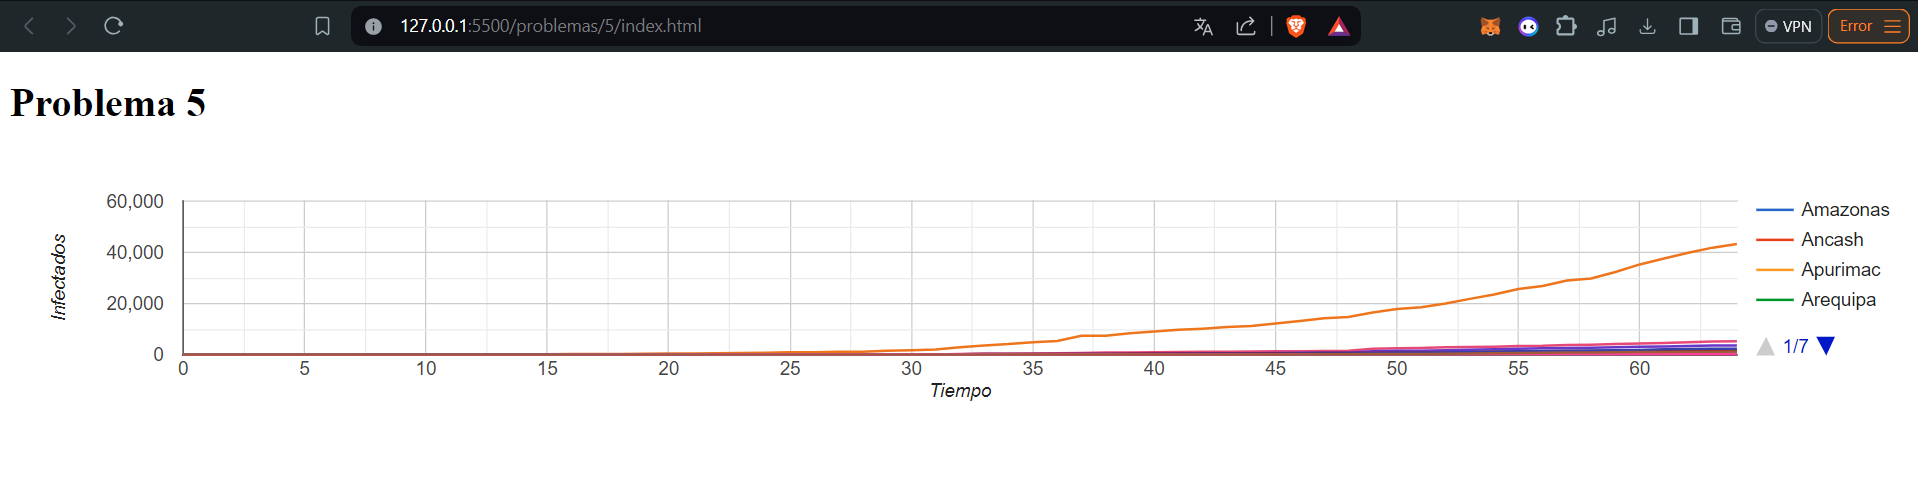
\includegraphics[width=0.8\textwidth,keepaspectratio]{PROBLEMA5.png}
            \newline \newline \newline

            \item Visualice un gráfico comparativo del crecimiento en regiones excepto Lima y Callao
            
            \begin{lstlisting}[language=JavaScript, caption=PROBLEMA6-INDEX]
<!DOCTYPE html>
<html lang="en">
<head>
  <meta charset="UTF-8">
  <meta name="viewport" content="width=device-width, initial-scale=1.0">
  <title>Problema 6</title>
  <script type="text/javascript" src="https://www.gstatic.com/charts/loader.js"></script>
</head>
<body>
  <h1>Problema 6</h1>
  <div id="chart_div"></div>
  <script src="./script.js"></script>
</body>
</html>
            \end{lstlisting}  

            \begin{lstlisting}[language=JavaScript, caption=PROBLEMA6-SCRIPT]
const $container = document.getElementById('container');

const xhr = new XMLHttpRequest(); 

xhr.open('GET', 'http://localhost:8000/data', true);
xhr.onreadystatechange = function () {
  if(xhr.readyState === 4 && xhr.status === 200) {
    const json = JSON.parse(xhr.responseText);
    
    const regionesExcluidas = ['Lima', 'Callao'];
    const regionesFiltradas = json.filter(region => !regionesExcluidas.includes(region.region));

    const datos = regionesFiltradas.map(region => {
      const confirmados = region.confirmed.map(entry => Number(entry.value));
      return { nombre: region.region, confirmados: confirmados };
    });

    google.charts.load('current', {packages: ['corechart', 'line']});
    google.charts.setOnLoadCallback(() => drawChart(datos));

    function drawChart(datos) {
      var data = new google.visualization.DataTable();
      data.addColumn('number', 'Días');
      

      datos.forEach(region => {
        data.addColumn('number', region.nombre);
      });

      const maxLength = datos.reduce((max, region) => Math.max(max, region.confirmados.length), 0);

      const rows = [];
      for (let i = 0; i < maxLength; i++) {
        const row = [i];
        datos.forEach(region => {
          row.push(region.confirmados[i] || null);
        });
        rows.push(row);
      }
      data.addRows(rows);

      var options = {
        hAxis: {
          title: 'Días'
        },
        vAxis: {
          title: 'Confirmados'
        }
      };

      var chart = new google.visualization.LineChart(document.getElementById('chart_div'));

      chart.draw(data, options);
    }
  }
}

xhr.send();
            \end{lstlisting}  

            \newline \newline \newline
            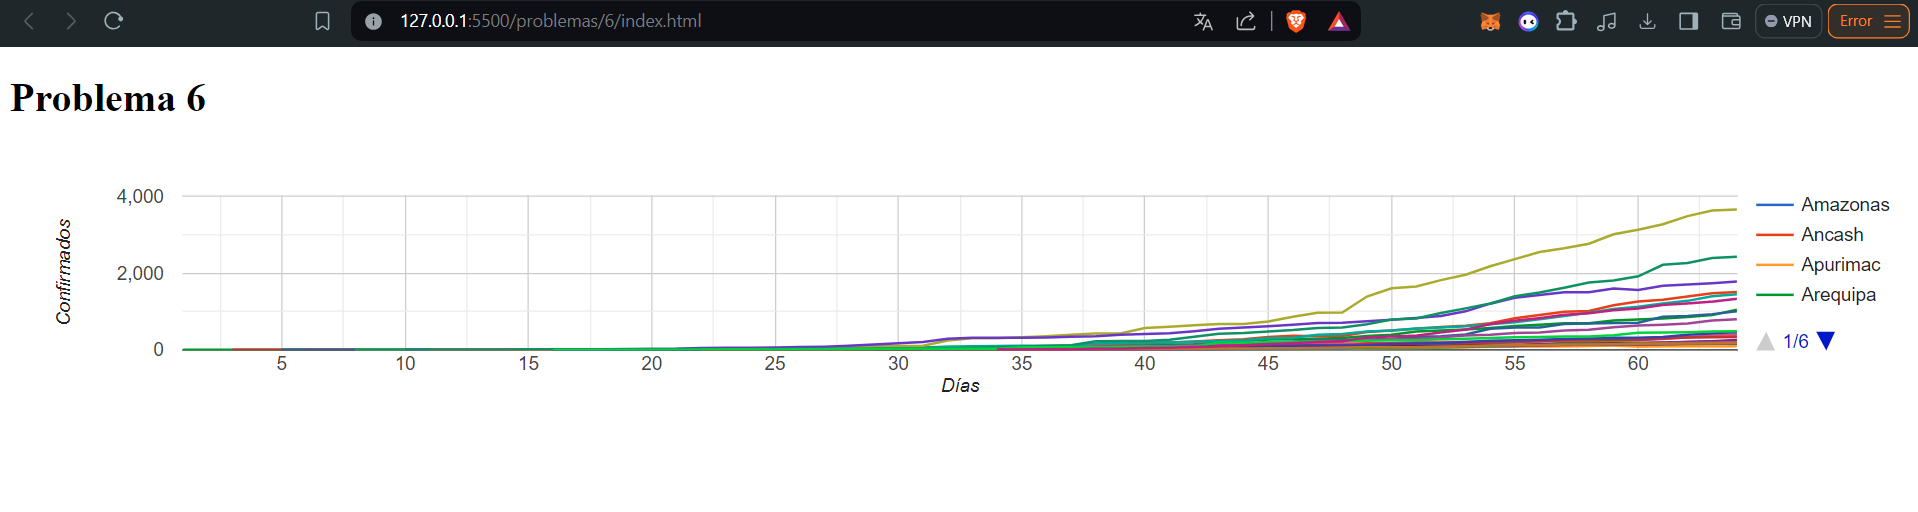
\includegraphics[width=0.8\textwidth,keepaspectratio]{PROBLEMA6.png}
            \newline \newline \newline

            \item Haga gráficos comparativos entre regiones elegidas por el usuario.
            
            \begin{lstlisting}[language=JavaScript, caption=PROBLEMA7-INDEX]
<!DOCTYPE html>
<html lang="en">
<head>
  <meta charset="UTF-8">
  <meta name="viewport" content="width=device-width, initial-scale=1.0">
  <title>Comparación de Regiones</title>
  <script src="https://ajax.googleapis.com/ajax/libs/jquery/3.5.1/jquery.min.js"></script>
  <script type="text/javascript" src="https://www.gstatic.com/charts/loader.js"></script>
</head>
<body>
  <h1>Problema 7: Comparación de Regiones</h1>
  <div>
    <label for="region1">Seleccione la primera región:</label>
    <select id="region1">

    </select>
  </div>
  <div>
    <label for="region2">Seleccione la segunda región:</label>
    <select id="region2">

    </select>
  </div>
  <div id="chart_div" style="width: 100%; height: 500px;"></div>
  <script src="./script.js"></script>
</body>
</html>
            \end{lstlisting}  

            \begin{lstlisting}[language=JavaScript, caption=PROBLEMA7-SCRIPT]
$(document).ready(function(){
  const xhr = new XMLHttpRequest(); 

  xhr.open('GET', 'http://localhost:8000/data', true);
  xhr.onreadystatechange = function () {
    if(xhr.readyState === 4 && xhr.status === 200) {
      const json = JSON.parse(xhr.responseText);
      const regiones = json.map(region => region.region);

      const $region1Select = $('#region1');
      const $region2Select = $('#region2');

      regiones.forEach(region => {
        $region1Select.append(`<option value="${region}">${region}</option>`);
        $region2Select.append(`<option value="${region}">${region}</option>`);
      });

      $region1Select.add($region2Select).change(function() {
        const region1 = $region1Select.val();
        const region2 = $region2Select.val();
        drawChart(json, region1, region2);
      }).change(); 
    }
  }

  xhr.send();

  function drawChart(json, region1, region2) {
    const lima = json.find(region => region.region === region1);
    const callao = json.find(region => region.region === region2);

    google.charts.load('current', {packages: ['corechart', 'line']});
    google.charts.setOnLoadCallback(function() {
      var data = new google.visualization.DataTable();
      data.addColumn('number', 'Días');
      data.addColumn('number', region1);
      data.addColumn('number', region2);

      const rows = [];
      const maxLength = Math.max(lima.confirmed.length, callao.confirmed.length);
      for(let i = 0; i < maxLength; i++) {
        const row = [i];
        row.push(Number(lima.confirmed[i]?.value || 0));
        row.push(Number(callao.confirmed[i]?.value || 0));
        rows.push(row);
      }

      data.addRows(rows);

      var options = {
        hAxis: {
          title: 'Tiempo'
        },
        vAxis: {
          title: 'Infectados'
        }
      };

      var chart = new google.visualization.LineChart(document.getElementById('chart_div'));

      chart.draw(data, options);
    });
  }
});
            \end{lstlisting}  

            \newline \newline \newline
            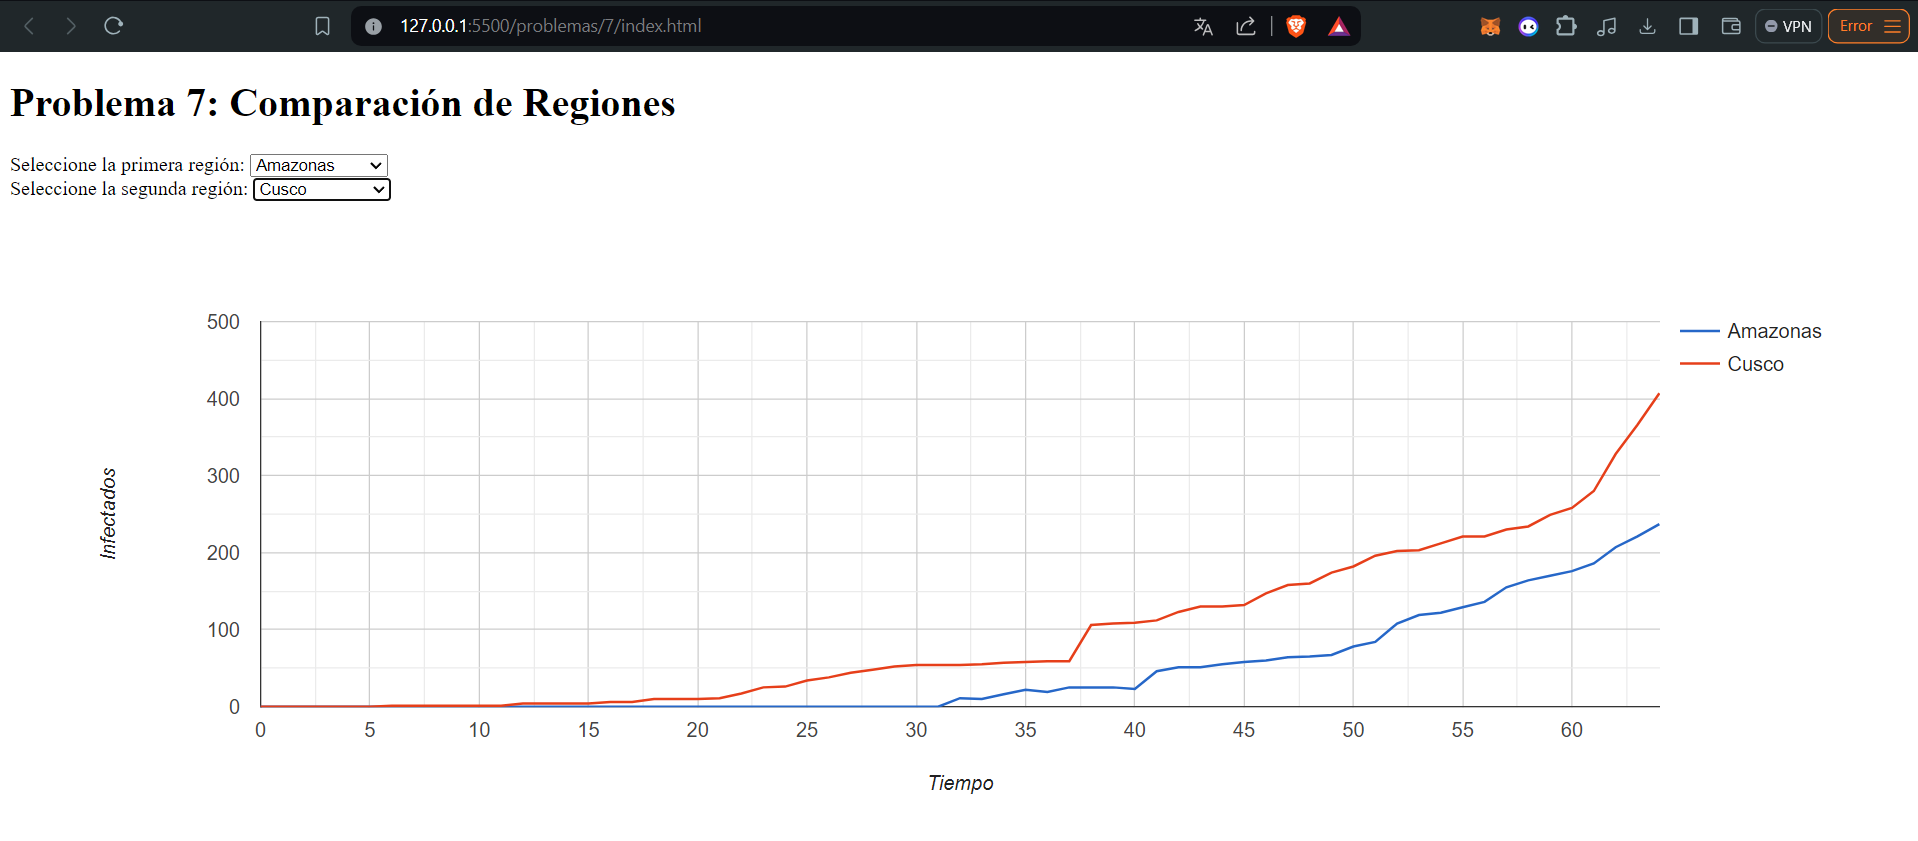
\includegraphics[width=0.8\textwidth,keepaspectratio]{PROBLEMA7.png}
            \newline \newline \newline

            \item Visualice un gráfico comparativo del crecimiento en regiones excepto Lima y Callao, mostrando el número de confirmados por cada día.
            
            \begin{lstlisting}[language=JavaScript, caption=PROBLEMA8-INDEX]
<!DOCTYPE html>
<html lang="en">
<head>
  <meta charset="UTF-8">
  <meta name="viewport" content="width=device-width, initial-scale=1.0">
  <title>Problema 8</title>
  <script type="text/javascript" src="https://www.gstatic.com/charts/loader.js"></script>
</head>
<body>
  <h1>Problema 8</h1>
  <div id="chart_div">  </div>
  <script src="./script.js"></script>
</body>
</html>
            \end{lstlisting}  

            \begin{lstlisting}[language=JavaScript, caption=PROBLEMA8-SCRIPT]
const $container = document.getElementById('container');

const xhr = new XMLHttpRequest(); 

xhr.open('GET', 'http://localhost:8000/data', true);
xhr.onreadystatechange = function () {
  if(xhr.readyState === 4 && xhr.status === 200) {
    const json = JSON.parse(xhr.responseText);
    
    const noLimaCallao = json.filter((region) => region.region !== 'Lima' && region.region !== 'Callao');

    google.charts.load('current', {packages: ['corechart', 'line']});
    google.charts.setOnLoadCallback(drawBasic);

    function drawBasic() {
      var data = new google.visualization.DataTable();
      data.addColumn('number', 'X');
 
      noLimaCallao.forEach((region) => {
        data.addColumn('number', region.region);
      })

      const rows = [];
      for(let i = 0; i < noLimaCallao[0].confirmed.length; i += 1) {
        const row = [i];
        noLimaCallao.forEach((region) => {
          row.push(Number(region.confirmed[i].value));
        })
        rows.push(row);
      }

      data.addRows(rows);

      var options = {
        hAxis: {
          title: 'Tiempo'
        },
        vAxis: {
          title: 'Infectados'
        }
      };

      var chart = new google.visualization.LineChart(document.getElementById('chart_div'));

      chart.draw(data, options);
    }
  }
}

xhr.send();
            \end{lstlisting}  

            \newline \newline \newline
            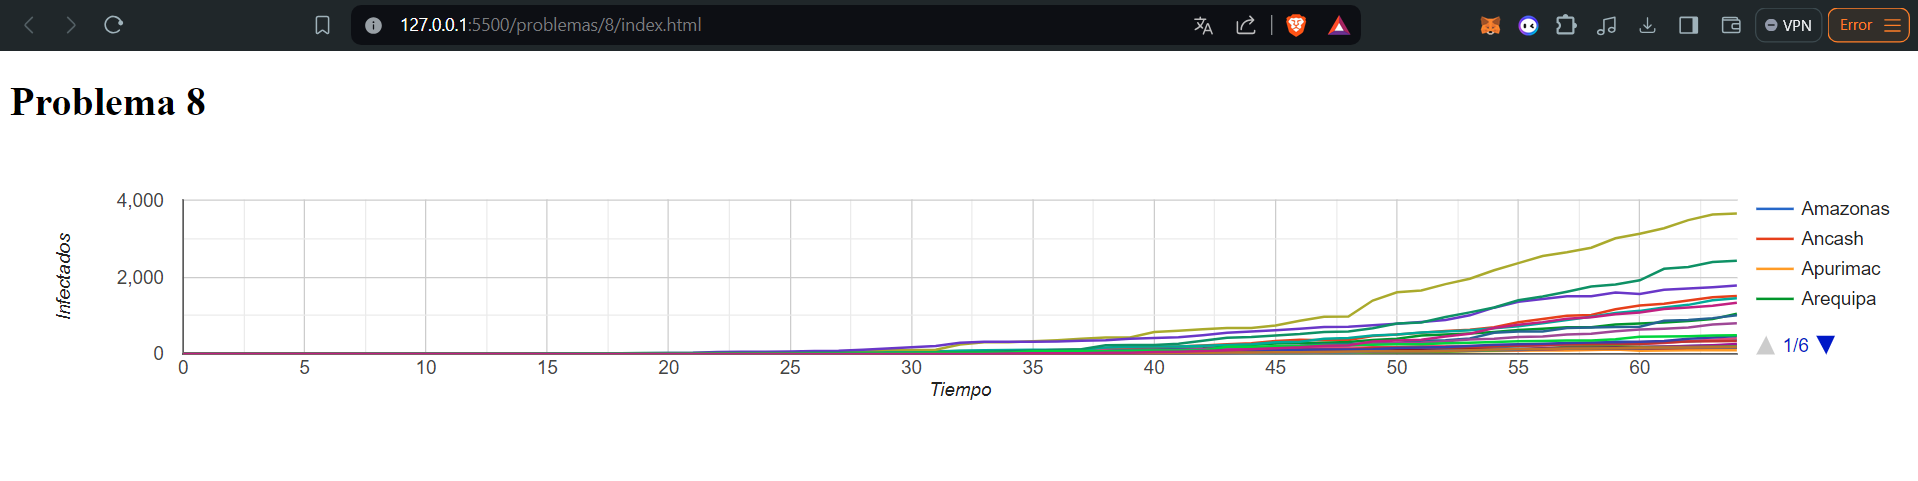
\includegraphics[width=0.9\textwidth,keepaspectratio]{PROBLEMA8.png}  
            
	\end{itemize}	
    \clearpage

	\section{\textcolor{red}{Rúbricas}}
	
	\subsection{\textcolor{red}{Entregable Informe}}
	\begin{table}[H]
		\caption{Tipo de Informe}
		\setlength{\tabcolsep}{0.5em} % for the horizontal padding
		{\renewcommand{\arraystretch}{1.5}% for the vertical padding
		\begin{tabular}{|p{3cm}|p{12cm}|}
			\hline
			\multicolumn{2}{|c|}{\textbf{\textcolor{red}{Informe}}}  \\
			\hline 
			\textbf{\textcolor{red}{Latex}} & \textcolor{blue}{El informe está en formato PDF desde Latex,  con un formato limpio (buena presentación) y facil de leer.}   \\ 
			\hline 
			
			
		\end{tabular}
	}
	\end{table}
	

	
	\subsection{\textcolor{red}{Rúbrica para el contenido del Informe y demostración}}
	\begin{itemize}			
		\item El alumno debe marcar o dejar en blanco en celdas de la columna \textbf{Checklist} si cumplio con el ítem correspondiente.
		\item Si un alumno supera la fecha de entrega,  su calificación será sobre la nota mínima aprobada, siempre y cuando cumpla con todos lo items.
		\item El alumno debe autocalificarse en la columna \textbf{Estudiante} de acuerdo a la siguiente tabla:
	
		\begin{table}[ht]
			\caption{Niveles de desempeño}
			\begin{center}
			\begin{tabular}{ccccc}
    			\hline
    			 & \multicolumn{4}{c}{Nivel}\\
    			\cline{1-5}
    			\textbf{Puntos} & Insatisfactorio 25\%& En Proceso 50\% & Satisfactorio 75\% & Sobresaliente 100\%\\
    			\textbf{2.0}&0.5&1.0&1.5&2.0\\
    			\textbf{4.0}&1.0&2.0&3.0&4.0\\
    		\hline
			\end{tabular}
		\end{center}
	\end{table}	
	
	\end{itemize}
	
	\begin{table}[H]
		\caption{Rúbrica para contenido del Informe y demostración}
		\setlength{\tabcolsep}{0.5em} % for the horizontal padding
		{\renewcommand{\arraystretch}{1.5}% for the vertical padding
		%\begin{center}
		\begin{tabular}{|p{2.7cm}|p{7cm}|x{1.3cm}|p{1.2cm}|p{1.5cm}|p{1.1cm}|}
			\hline
    		\multicolumn{2}{|c|}{Contenido y demostración} & Puntos & Checklist & Estudiante & Profesor\\
			\hline
			\textbf{1. GitHub} & Hay enlace URL activo del directorio para el  laboratorio hacia su repositorio GitHub con código fuente terminado y fácil de revisar. &2 &X &2 & \\ 
			\hline
			\textbf{2. Commits} &  Hay capturas de pantalla de los commits más importantes con sus explicaciones detalladas. (El profesor puede preguntar para refrendar calificación). &4 &X &2 &  \\ 
			\hline 
			\textbf{3. Código fuente} &  Hay porciones de código fuente importantes con numeración y explicaciones detalladas de sus funciones. &2 &X &2 & \\ 
			\hline 
			\textbf{4. Ejecución} & Se incluyen ejecuciones/pruebas del código fuente  explicadas gradualmente. &2 &X &1 & \\ 
			\hline			
			\textbf{5. Pregunta} & Se responde con completitud a la pregunta formulada en la tarea.  (El profesor puede preguntar para refrendar calificación).  &2 &X &2 & \\ 
			\hline	
			\textbf{6. Fechas} & Las fechas de modificación del código fuente estan dentro de los plazos de fecha de entrega establecidos. &2 &X &2 & \\ 
			\hline 
			\textbf{7. Ortografía} & El documento no muestra errores ortográficos. &2 &X &2 & \\ 
			\hline 
			\textbf{8. Madurez} & El Informe muestra de manera general una evolución de la madurez del código fuente,  explicaciones puntuales pero precisas y un acabado impecable.   (El profesor puede preguntar para refrendar calificación).  &4 &X &4 & \\ 
			\hline
			\multicolumn{2}{|c|}{\textbf{Total}} &20 & &17 & \\ 
			\hline
		\end{tabular}
		%\end{center}
		%\label{tab:multicol}
		}
	\end{table}
	
\clearpage
	
	
%\clearpage
%\bibliographystyle{apalike}
%\bibliographystyle{IEEEtranN}
%\bibliography{bibliography}
			
\end{document}
